\documentclass{projdoc}

\usepackage{eso-pic}

\title{Software Design}

\begin{document}
\tablestables
\newpage

\section{Introduction}

This document outlines the design and development process of the cr\^epe game engine,
detailing the key decisions made during its creation. The primary goal of this engine
is to offer a streamlined, Unity-like experience tailored for developing 2D games
similar to Jetpack Joyride.

The cr\^epe engine is designed to ease the transition for developers familiar with
Unity, ensuring minimal friction when switching platforms. Our aim is to preserve
many of Unity's core features while introducing a lightweight and open-source
alternative, licensed under the MIT License.

The engine is primarily aimed at indie developers who have prior experience with
Unity and are looking for a flexible, cost-effective solution with familiar
workflows.

\section{Overview}

As described above, the cr\^epe game engine's goal is to offer a Unity-like
experience tailored for developing 2D games similar to Jetpack Joyride. That is why
Jetpack Joyride and Unity provided the main inputs for this game engine design.
Firstly, a quick overview will be given of the Unity game engine, in particular the
\gls{ecs}. Secondly, this Overview will quickly talk you through some of the most
important parts of the game engine, and why these parts are needed to create the
Jetpack Joyride game.

\subsection{ECS}

The Unity game engine is structured using the Entity Component System (\gls{ecs}) (as
shown in \cref{fig:ecs-block-diagram}). The \gls{ecs} is made out of three main
subsystems, namely entities, components and systems. Entities are just IDs. An entity
is also called a GameObject in Unity and it is made out of one (or more) components.
Components are the classes that hold the data. The components determine what kind of
entity it is (e.g. an enemy, audio, and so on). Systems take care of the behavior of
the entities. Systems mainly read and write the enity's components data. The
\gls{ecs} clearly distinguishes the data (components) from the functionality
(systems).

\begin{figure}
	\centering
	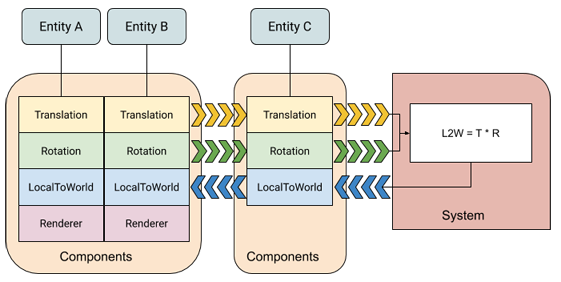
\includegraphics[width=0.5\textwidth]{img/ECSBlockDiagram.png}
	\caption{ECS design pattern}
	Source: \autocite{img:ecs-block-diag}
	\label{fig:ecs-block-diagram}
\end{figure}

The \gls{ecs} will also be used at the cr\^epe game engine. Everything (from the
protagonist and bullets to the walls and enemies) in the cr\^epe game engine will be
a GameObject (i.e.~entity). The game programmer must program his game by creating all
kind of GameObjects and placing them in one (or multiple) scenes, just like Unity.

\subsection{Jetpack Joyride}

Firstly, some background information about Jetpack Joyride. Jetpack Joyride is a
side-scrolling endless runner action video game created by Halfbrick Studios. The
protagonist is called Barry Steakfries, who the player controls as he steals a
bullet-powered jet pack from a top-secret laboratory
\autocite{wikipedia:jetpack-joyride}. A screenshot from the game can be seen in
\cref{fig:jetpack-joyride} (pleae be aware that the goal of this project is not to
create an exact replica of Jetpack Joyride, it is only used as a source of
inspiration).

\begin{figure}
	\centering
	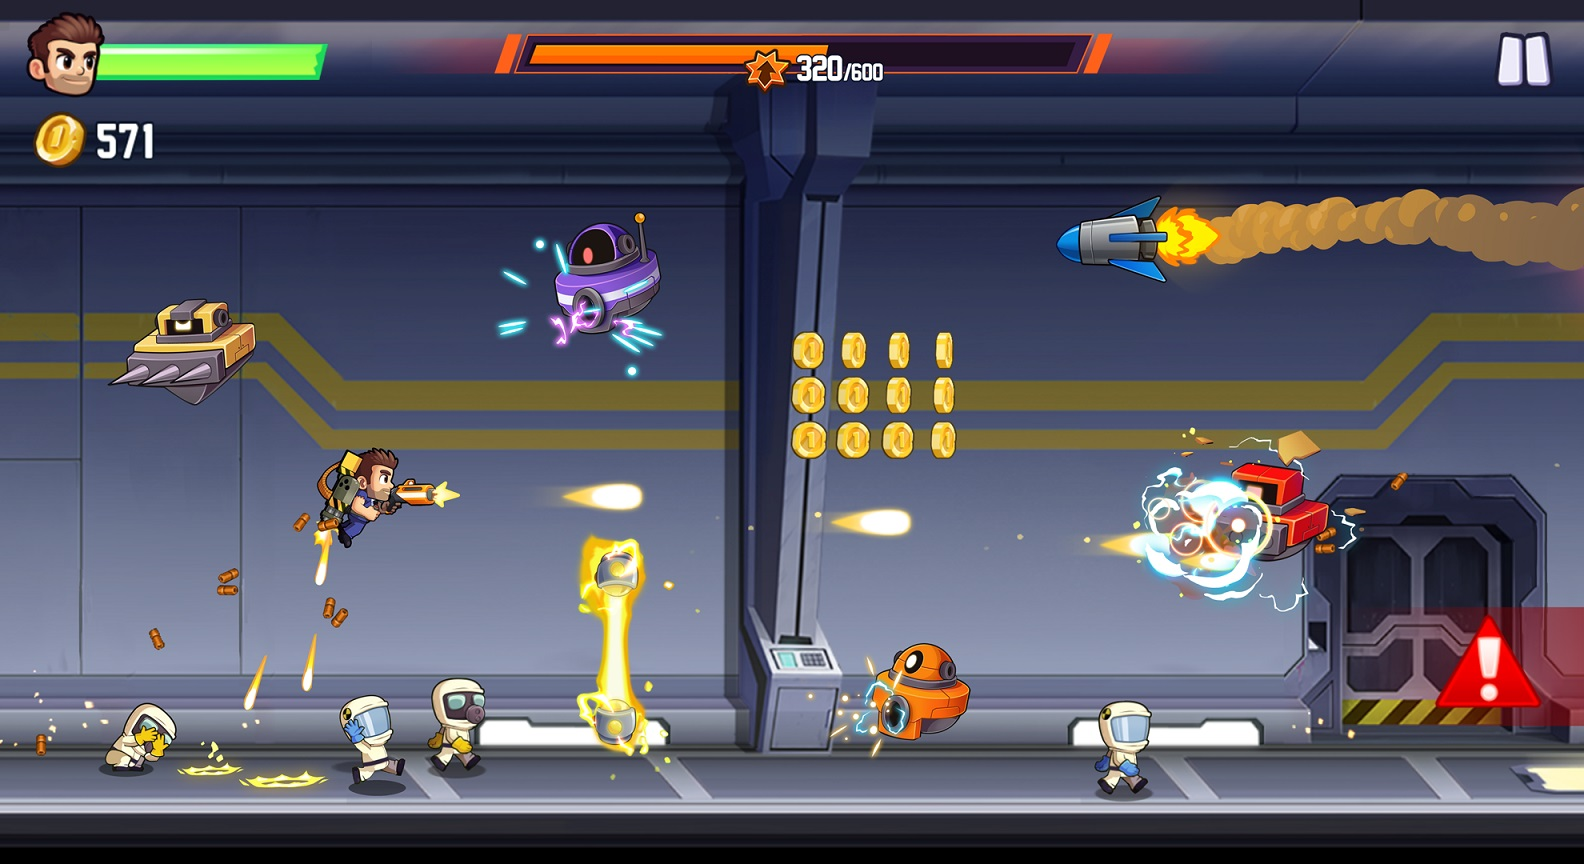
\includegraphics[width=0.5\textwidth]{img/JetpackJoyride.jpg}
	\caption{Jetpack Joyride}
	Source: \autocite{img:jetpack-joyride}
	\label{fig:jetpack-joyride}
\end{figure}

The protagonist wears a jetpack with which he can float in the air. The player must
avoid obstacles (such as lasers, missiles and zappers) by floating at the right
height. The player can control the protagonist's jetpack, thereby also controlling
the protagonist's height. The protagonist experiences gravity and other forces (like
the force from his jetpack pushing him upwards). These forces should be easily
programmable by the game programmer. That is why a physics system is needed in the
cr\^epe game engine. Only very limited/easy physics are needed for Jetpack Joyride,
that is why this is only supported by the cr\^epe game engine.

The protagonist must avoid obstacles. That is why the cr\^epe game engine should also
support a collision system. Again, only very limited/easy collision is needed for
Jetpack Joyride, that is why only very limited/easy collision is supported by the
cr\^epe game engine.

The game must, of course, also be visible to and playable by the user. A rendering
system will take care of rendering (displaying) the game and its GameObjects. An
input system will take care of all the inputs (mouse and keyboard).

Jetpack Joyride also offers audio. A system will take care of the audio in the
cr\^epe game engine.

Particles are very common in Jetpack Joyride, e.g. underneath the jetpack and behind
the rockets. Particles will be supported by the particle system.

The start of a scene is described in a scene. However, the game programmer might also
want to write game logic code which is running during the game (e.g. to switch to a
new scene or to perform a custom action at a collision). For these purposes, Unity
uses scripts. These scripts will also be supported by the cr\^epe game engine.

Finally, as an extra, replay functionality will be supported by the cr\^epe game
engine. A dedicated replay system will be used to support replay.

It turns out that a physics, collision, rendering, input, audio, particle, script,
and replay system are needed to create the Jetpack Joyride game. These systems form
the main part of the \gls{ecs}. The design of these eight systems in combination with
\gls{ecs}, will be briefly discussed in the next parts of this design document.

\section{Design}

\subsection{Game Loop}

\subsubsection{Problem statement}

A game loop is essential for maintaining a continuous flow of game actions, ensuring
that updates to game logic, physics, and rendering occur in a synchronized manner.
Without a game loop, the game would lack consistent timing, leading to unpredictable
behavior. The game loop is primarily responsible for two main tasks:\noparbreak
\begin{itemize}
	\item Updating all systems in the correct order
	\item Ensuring the game loop timer remains accurate
\end{itemize}

The game loop can be external where the user has the ability to update the systems
themselves or an intergrated game loop which is managed by the gameloop. Both of
these approaches have advantages and disadvantages when it comes to flexibility and
reliability.

\subsection{Texture}

The textures in cr\^epe game engine are represented by the \codeinline{Texture}
class. It is implemented as an \gls{facade} around the \gls{sdl} library.

\subsubsection{Architecture}

\Cref{fig:class-texture} shows a class diagram of the texture \gls{facade}. It
contains the following classes:\noparbreak
\begin{description}
	\item[SDLContext] This is a facade around the \codeinline{SDL2} library which is
		used around different parts of the engine, and is therefore implemented as a
		singleton. This class is friends with \codeinline{Texture},
		\codeinline{LoopManager}, \codeinline{RenderSystem} and
		\codeinline{AnimatorSystem}.
	\item[Texture] This is a wrapper around the \codeinline{SDL_Texture} class, and
		uses cr\^epe's \codeinline{Asset} class to load an Texture instead.
\end{description}

\begin{figure}
	\centering
	% TODO: export as vector format instead
	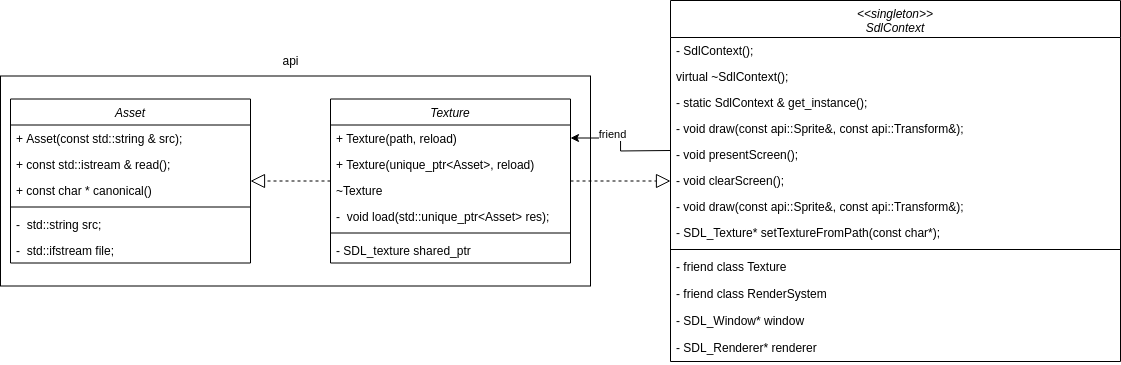
\includegraphics[width=\textwidth]{img/texture.png}
	\caption{User texture class diagram}
	\label{fig:class-texture}
\end{figure}

\subsection{AssetManager}

The AssetManager is a \gls{api} class that the user can use to make a
\codeinline{Asset} available from different scenes.

\subsubsection{Architecture}

\Cref{fig:class-assetmanager} shows a class diagram of the AssetManager. It contains
the following classes:\noparbreak
\begin{description}
	\item[AssetManager] is a Singleton class, meaning only one instance of this class
		exists throughout the application. This ensures a single point of access and
		control over asset management, simplifying resource handling and avoiding
		duplicated assets in memory.
\end{description}

\begin{figure}
	\centering
	% TODO: export as vector format instead
	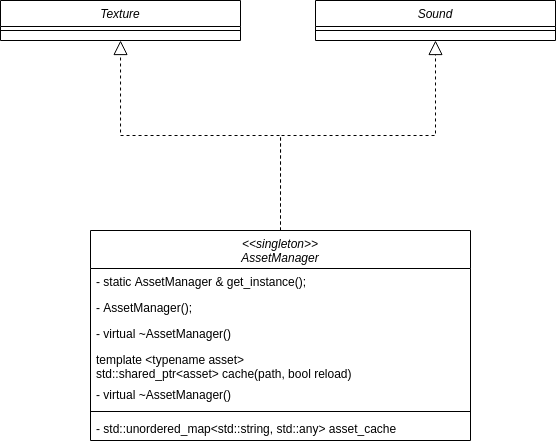
\includegraphics[width=0.5\textwidth]{img/AssesManager.png}
	\caption{User AssetManager class diagram}
	\label{fig:class-assetmanager}
\end{figure}

\subsection{Rendering}

Every game engine has an rendering structure to present all the different enities and
components on the screen.

\subsubsection{Architecture}

% TODO: anyone read this?
\Cref{fig:class-rendering} shows a class diagram of the RenderSystem. It contains the
following classes:\noparbreak
\begin{itemize}
	\item The system architecture is centered around rendering and component
		management, with the following key components:\noparbreak
		\begin{description}
			\item[\codeinline{System}] An interface class containing the virtual
				\codeinline{update()} function.
			\item[\codeinline{RenderSystem}] A derived class of \codeinline{System}
				responsible for rendering operations.
		\end{description}
	\item The \codeinline{System::get_instance()} function provides a static, singleton
		instance for managing system-wide operations.
	\item The \codeinline{RenderSystem} class implements various rendering
		functions:\noparbreak
		\begin{description}
			\item[\codeinline{sort_layers()}] Organizes the rendering layers.
			\item[\codeinline{clear_screen()}] Clears the screen prior to rendering.
			\item[\codeinline{update_sprites()}] Updates sprite positions and states.
			\item[\codeinline{update_camera()}] Manages the camera view.
			\item[\codeinline{present_screen()}] Presents the final rendered image to the
				screen.
		\end{description}
	\item The \codeinline{SdlContext} class, another singleton, manages the \gls{sdl}
		library
	\item Components are organized as follows:\noparbreak
		\begin{itemize}
			\item The \codeinline{Component} base class allows for generic handling of
				components.
			\item Derived component classes include:\noparbreak
				\begin{description}
					\item[\codeinline{Sprite}] Represents visual elements with attributes like
						\codeinline{sprite}, \codeinline{color}, \codeinline{flip},
						\codeinline{sortingLayer}, and \codeinline{orderInLayer}.
					\item[\codeinline{Transform}] Manages positional attributes, including
						\codeinline{position}, \codeinline{rotation}, and \codeinline{scale}.
				\end{description}
		\end{itemize}
	\item Both \codeinline{Sprite} and \codeinline{Transform} components provide a
		\codeinline{get_instances_max()} function to retrieve the maximum instance count.
\end{itemize}

\begin{figure}
	\centering
	% TODO: export as vector format instead
	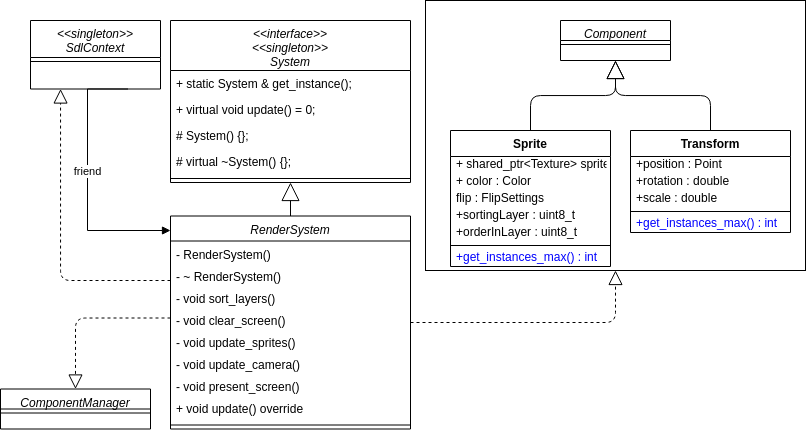
\includegraphics[width=\textwidth]{img/Rendering.png}
	\caption{System Rendering class diagram}
	\label{fig:class-rendering}
\end{figure}

\subsubsection{System}

\begin{figure}
	\centering
	% TODO: export as vector format instead
	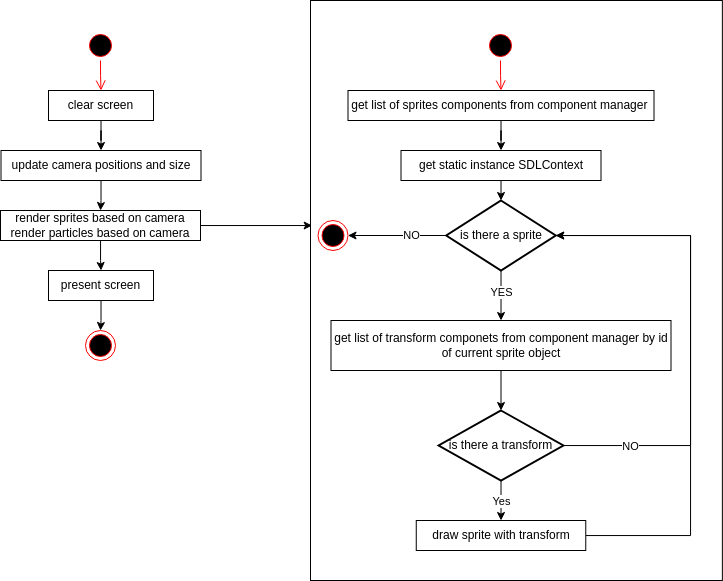
\includegraphics[width=\textwidth]{img/flowchart_rendering.png}
	\caption{System Rendering flowchart }
	\label{fig:class-renderingflowchart}
\end{figure}

\subsubsection{Architecture}

This engine uses an integrated game loop for the following reasons:\noparbreak
\begin{description}
	\item[Simplifies development] The user only needs to call \codeinline{startGame()}.
	\item[Ensures uniform system calls] Systems are always updated in the same order,
		reducing the likelihood of overwrites and undefined system behavior.
	\item[Provides a reliable timer update] The game loop timer is updated with each
		cycle, minimizing timing issues.
\end{description}

As seen in \cref{fig:gameloop-flow}, the game loop consists of multiple
steps:\noparbreak
\begin{description}
	\item[Update loop timer] The loop timer is updated, and the expected frame time is
		calculated.
	\item[Check events] Queued events are dispatched, and callback functions are
		executed accordingly.
	\item[Process input] The input system is called, and user inputs are processed.
	\item[Fixed update] A fixed loop for timing-sensitive systems, such as physics.
	\item[Update] A per-frame update for all necessary frame-dependent changes.
	\item[Render] The render system is called to display the current frame.
\end{description}

The game loop continues to call the fixed update function as long as there is
sufficient time. Delta time, calculated as the time between the last frame’s start
and the current frame, is used to measure the duration of each frame. This value is
converted into a time-based unit, enabling systems to create frame rate-independent
behavior.

Rendering and animations are handled on a per-frame basis. A delay, combined with
delta time calculation, ensures consistent visuals even at varying frame rates.
\Cref{gameloop-class} shows a \codeinline{TimerClass} using a singleton design
pattern, allowing access to \codeinline{deltaTime} throughout the system. The game
loop updates the timing and delta time in this class to keep it accurate.

The two main functions of the game loop are \codeinline{setup()} and
\codeinline{loop()}. \codeinline{setup()} handles all startup procedures and is
called only once when the game begins. The \codeinline{loop()} function repeats as
long as the game is running.

The code example below shows how to start the game engine/game:\noparbreak
\begin{blockcode}
Gameloop loop;
loop.start();
\end{blockcode}

% FIXME: not a technical reference
This code calls both \codeinline{setup()} and \codeinline{loop()}, starting the game
loop timer. The current frame’s delta time can be accessed using
\codeinline{LoopTimer::getInstance().getDeltaTime()}, which returns the expected
frame time.

\begin{figure}
	\centering
	\includepumldiag{img/gameloop-flow.puml}
	\caption{Game loop flowchart diagram}
	\label{fig:gameloop-flow}
\end{figure}

\begin{figure}
	\centering
	\includepumldiag{img/gameloop-class.puml}
	\caption{Gameloop flowchart diagram}
	\label{fig:gameloop-class}
\end{figure}

\subsection{Event system}

\subsubsection{Problem Statement}

The game engine utilizes the \gls{ecs} architecture, where components store data, and
systems process that data to apply changes. Each system is responsible for managing a
specific domain, such as physics in the physics system and rendering in the rendering
system. To facilitate communication between systems without introducing direct
dependencies, a method of inter-system communication is required to maintain loose
coupling. Additionally, a mechanism that allows one object's trigger to manipulate
adn affect multiple other objects is beneficial for game developers, providing
greater flexibility in designing interactions within the game.

\subsubsection{Architecture}

The sollution to connect the various systems and BehaviorScripts together without
inducing high coupling is an event system that facilitates communication between
systems and BehaviorScripts using various types of events. The event system includes
several pre-defined events, all derived from a parent Event class, capable of
handling user input and application-level events, such as window resizing.
Furthermore, a specific event is designated for the collision handler within the
physics system, which can be triggered when two objects collide. The event system
also allows developers to create custom events, such as "onPlayerDeath," and assign
callback functions that execute when the event is triggered.

\begin{figure}
	\centering
	% TODO: export as vector format instead
	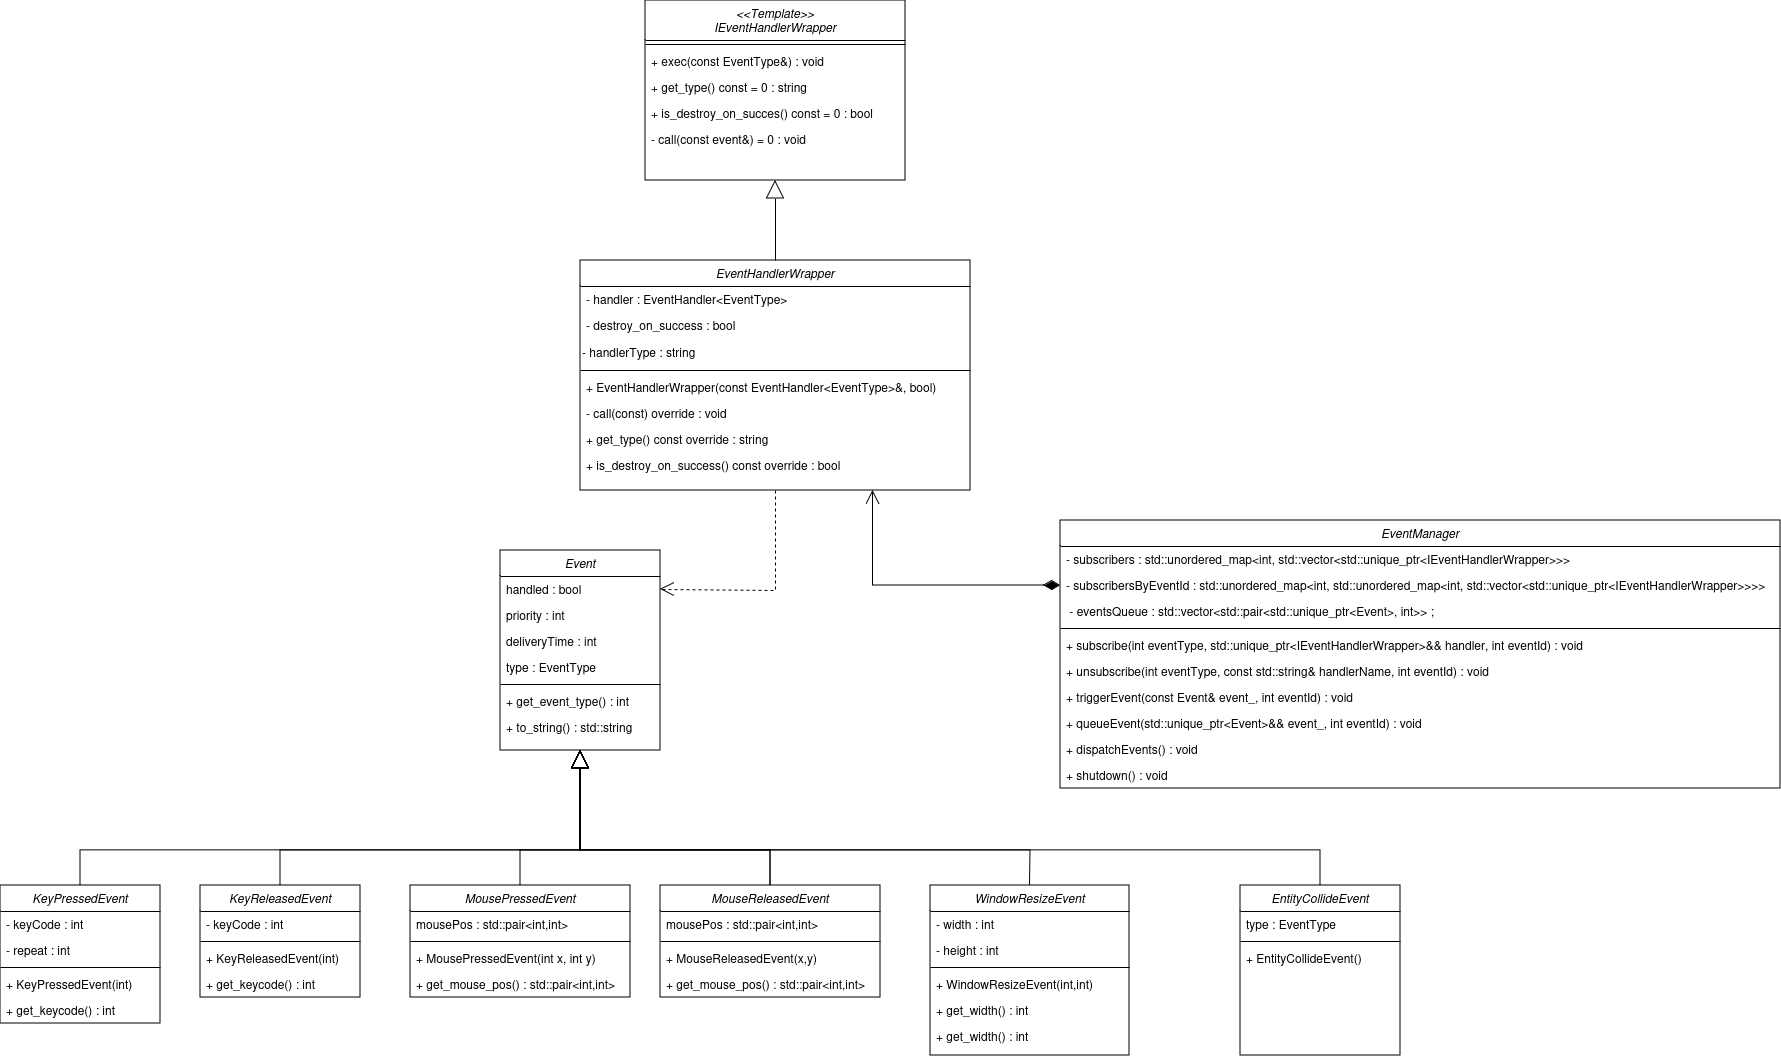
\includegraphics[width=\linewidth]{img/event-uml.drawio.png}
	\caption{Event system class diagram}
	\label{fig:event-uml}
\end{figure}

The event system as seen in \cref{fig:event-uml} includes several parts such
as:\noparbreak
\begin{description}
	\item[eventManager] The manager has the functions to
		subscribe/trigger/queue/dispatch events. It also stores all callback functions
		corresponding to specific event. The manager is a singleton and can therefor only
		exist once so all events are stored in one place.
	\item[IEventWrapper] This is a EventWrapper \emph{interface} which is used to store
		all the different templated eventshandlers in one map in the event manager. this
		wrapper contains the logic to convert the parent class \emph{event} to the
		correct subclasses. It also contains a variable onSuccessDestroy which can be set
		to destroy the callback call onces completed. This can be used to make a one time
		only event.
	\item[Event] This is the parent class where all specific event classes are derived
		from. Each event contains a---
		\begin{itemize}
			% TODO: the design document is not a technical reference, so implementation
			% details shouldn't even be in here. Also, are getter functions used to set
			% things nowadays?
			\item \emph{\codeinline{static std::uint32_t getStaticEventType()}} to set type
				during compiling.
			\item \emph{\codeinline{virtual std::uint32_t getEventType() const override }}
				function to manage the type conversion during runtime.
		\end{itemize}
		Other functions can be freely added when creating a custom function. When an
		event is triggered a specific derived class must be used to indicate which event
		is triggered. A reference to this event is then transfered to all callback
		functions subscribed.
	\item[IKeyListener] This is an interface designed to match the API. By deriving
		from this interface the game developer can override the key event functions to
		add their own functionality. The derived class will immediately be subscribed to
		the EventManager and will Unsubscibe when deleted.
	\item[IMouseListener] Like the IKeyListener this is also an interface to interact
		with the eventManager. The derived classes from this interface handle various
		mouse related events. These events are triggered when the mouse is
		clicked/pressed/released or moved.
\end{description}

The gamedeveloper can interact with the EventManager using the following
functions:\noparbreak
\begin{description}
	\item[Subscribe] This subscribes a function pointer or lambda function to a given
		event. The function can be subscribed either to all event triggers or a specifc
		ID.
	\item[Trigger] This triggers a given event and all callbacks correlating to this
		event are executed immediately.
	\item[Queue event] This queues an event to be executed at a fixed time during the
		gameloop.
	\item[Unsubscibe] This removes the callback function from the event and it will no
		longer be executed.
\end{description}

\Cref{fig:event-seq} shows that when a specific function is triggered or dispatched
using the callback(eventHandler) is executed.

\begin{figure}
	\centering
	\includepumldiag{img/event-sequence.puml}
	\caption{Sequence diagram for event calling}
	\label{fig:event-seq}
\end{figure}

% \subsection{Physics}

\subsection{Rendering}

\subsection{Scripting}

The scripting interface was designed around a `target' \gls{api} (described by
\cref{req:script:interface,req:script:user-class,req:script:direct-instance,req:script:direct-run}).
An example of this \gls{api} is shown below:\noparbreak

\begin{blockcode}
class MyScript : public BehaviorScript {
	void update() {
		// update code here
	}
	// init() also exists, but is empty by default
};

{ // in scene initialization
	GameObject & obj = ...;
	obj.add_component<MyScript>();
}
\end{blockcode}

The above call to \codeinline{GameObject::add_component} cannot work correctly
without significantly increasing the complexity of the component manager, so the
following restrictions were taken into account when creating the script system
architecture:\noparbreak

\begin{itemize}
	\item The first template parameter passed to \codeinline{GameObject::add_component}
		\emph{must} be a base `script \emph{component}' class, so each derived user
		script class is instantiated in the same generic script list.
	\item C++ does not allow passing types (i.e.~\codeinline{MyScript} in this case) as
		function parameters, so a function call like
		\codeinline{add_component<BehaviorScript>(MyScript)} cannot be realized.
\end{itemize}

\subsubsection{Architecture}
\label{sec:scripts:architecture}

The restrictions detailed at the start of this section are mitigated as
follows:\noparbreak

\begin{itemize}
	\item User scripts are split into two classes---
		\begin{enumerate}
			\item a script \emph{interface} class (\codeinline{Script})
			\item a script \emph{component} class (\codeinline{BehaviorScript})
		\end{enumerate}
	\item \codeinline{GameObject::add_component} receives the script \emph{component}
		as template parameter
	\item \codeinline{GameObject::add_component} now always returns a reference to the
		component instance
	\item The script component class has a setter function that takes a template
		parameter for classes derived from the base script \emph{interface} class
\end{itemize}

\Cref{fig:class-scripts} shows the resulting structure as a class diagram. It
contains the following classes:\noparbreak
\begin{description}
	\item[Script] This is the script \emph{interface}, and is used by the game
		programmer to create derived script classes. All virtual methods in this class
		have an empty implementation by default, and are optionally implemented by the
		game programmer.

		This class' virtual methods are protected by default, and a friend relation to
		\codeinline{ScriptSystem} is used to ensure only \codeinline{ScriptSystem} is
		able to call these methods.

		Only classes derived from \codeinline{Script} can be used with
		\codeinline{BehaviorScript::set_script}'s template parameter \codeinline{T}. This
		function returns a reference to the \codeinline{BehaviorScript} instance it was
		called on so it can be chained after the call to
		\codeinline{GameObject::add_component}.

		\codeinline{Script} also has a reference to its parent
		\codeinline{BehaviorScript} instance so components can easily be retrieved using
		the component manager.
	\item[BehaviorScript]
		This is the script \emph{component}, and is given as the template parameter to
		\codeinline{GameObject::add_component}.

		This class also uses a friend relation to \codeinline{ScriptSystem} to restrict
		access to its private reference member \codeinline{script}.
	\item[ScriptSystem] This is the system class that runs the methods implemented in
		the derivative instances of \codeinline{Script}. Described further in
		\cref{sec:scripts:sytem}.
\end{description}

\begin{figure}
	\centering
	\includepumldiag{img/class-scripts.puml}
	\caption{User script class diagram}
	\label{fig:class-scripts}
\end{figure}

\subsubsection{System}
\label{sec:scripts:sytem}

Because most of the complexity in the scripting interface comes from the containers
described in \cref{sec:scripts:architecture}, the script system class itself is
relatively simple. The script system provides a method
\codeinline{ScriptSystem::update} that calls all active script's update functions.

Because of the limitation that types cannot be passed as parameters in C++, the
user-defined script class (derived from \codeinline{Script}) can not directly be
instantiated when adding the component to the component manager. To work around this
limitation, the method \codeinline{BehaviorScript::set_script} was created. This
results in the possibility that an instance of \codeinline{BehaviorScript} does not
reference an instance of \codeinline{Script}. In addition to the non-active script
components, the script system skips over these `invalid' instances. This is
illustrated in \cref{fig:activity-scripts}.

\begin{figure}
	\centering
	\includepumldiag{img/activity-scripts.puml}
	\caption{Script system update method}
	\label{fig:activity-scripts}
\end{figure}

A \gls{poc} for the script system is shown in \cref{poc:scripts}.

\subsection{Audio}

Since writing a custom real-time audio mixing engine is outside the scope of this
project\mref and C++ does not provide a built-in cross-platform audio \gls{api}, the
audio system inside the cr\^epe engine is implemented as a \gls{facade} around an
existing audio library.

\subsubsection{Libraries}
\label{sec:audio:libs}

This subsection compares various standalone audio libraries for suitability. After
searching for libraries (search terms: `dynamic/adaptive audio', `real-time audio',
`audio library', `game audio engine'), several libraries were found. These libraries
were checked against the audio engine requirements \autocite{crepe:requirements} and
then tested by writing the same benchmark-style \gls{poc} using the remaining
qualifying libraries. These \glspl{poc} are detailed in \cref{poc:audio}.

Of these libraries the following were determined to be unsuitable for use in this
project:\noparbreak
\begin{description}
	\item[FMOD \autocite{lib:fmod}] Is proprietary (violates \cref{req:lib:license}).
	\item[PortAudio \autocite{lib:portaudio}] Does not handle mixing.
	\item[miniaudio \autocite{lib:miniaudio}] Tested by implementing a \gls{poc}, but
		dropped due to very limited codec support (WAV, MP3 and FLAC only); Also does not
		have an \gls{api} reference (only programming manual).
	\item[YSE \autocite{lib:yse}] Attempted to write \gls{poc}, but CMake configuration
		in repository is broken; This project seems to have been abandoned.
\end{description}

The only library that remained after these tests is SoLoud \autocite{lib:soloud}. It
is Zlib/LibPng licensed and provides a high-level object-oriented C++ \gls{api}.
\Cref{sec:audio:architecture} describes the \gls{facade} written for this library.

\subsubsection{Architecture}
\label{sec:audio:architecture}

\Cref{fig:class-audio-facade} shows a class diagram of the audio \gls{facade}. It
contains the following classes:
\begin{description}
	\item[SoundContext] This is a wrapper around the \codeinline{SoLoud::soloud}
		`engine' class, and is therefore implemented as a singleton. This ensures the
		audio engine is initialized before \codeinline{Sound} is able to use it.

		This class is friends with \codeinline{Sound}, so only \codeinline{Sound} is able
		to get the \codeinline{SoundContext} instance.
	\item[Sound] This is a wrapper around the \codeinline{SoLoud::Wav} class, and uses
		cr\^epe's \codeinline{Asset} class to load an audio sample instead.
\end{description}

\begin{figure}
	\centering
	\includepumldiag{img/facade-audio.puml}
	\caption{Audio \glsfmtshort{facade} class diagram}
	\label{fig:class-audio-facade}
\end{figure}

A \gls{poc} for the final Audio \gls{facade} is also showcased in \cref{poc:audio}.

% \subsection{Save manager}
%
% The save manager \gls{api} is designed to give the game programmer an easy to use
% interface for retrieving and storing game-specific data (\cref{req:savemgr}).
%
% Because the engine validation app only stores statistics and highscores, the save
% manager is not required to support loading different save files
% (\cref{req:savemgr:multi-file}), nor storing complicated data types
% (\cref{req:savemgr:types-custom}). The save manager only supports storing simple
% types (\cref{req:savemgr:types-scalar,req:savemgr:types-string}).
%
% In order to reduce complexity for the game programmer further, the following
% requirements were also set:\noparbreak
%
% \begin{itemize}
% 	\item Prevent data loss in the case of crashes (\cref{req:savemgr:journalling})
% 	\item Handle opening/closing/flushing of the underlying file automatically
% 		(\cref{req:savemgr:file-manage})
% 	\item Save file variables are uniquely identified (\cref{req:savemgr:var-key})
% \end{itemize}
%
% \subsubsection{Architecture}
% \label{sec:savemgr:architecture}
%
% \begin{figure}
% 	\centering
% 	\includepumldiag{img/class-savemgr.puml}
% 	\caption{Save manager class diagram}
% 	\label{fig:class-savemgr}
% \end{figure}
%
% In order to realize \cref{req:savemgr:journalling,req:savemgr:var-key}, a third-party
% key-value database library is used.

\subsection{Global configuration interface}

Because the game programmer only has access to interfaces within the public \gls{api}
namespace (\codeinline{crepe::api}), they would not be able to configure aspects of
engine-internal components. To work around this access restriction, a global
interface was made that stores arbitrary data, which can be accessed both internally
and via the public \gls{api}.

\subsubsection{Architecture}
\label{sec:config:architecture}

The global configuration interface consists of a single singleton class that can be
accessed globally (see \cref{fig:class-config}). This class holds several anonymous
structs, which are used to organize options per system or engine component.

\begin{figure}
	\centering
	\includepumldiag{img/class-config.puml}
	\caption{Global configuration interface class diagram}
	\label{fig:class-config}
\end{figure}

% \subsection{Input}

% \subsection{Physics}

\appendix

\section{Proof-of-concepts}

The full (documented) source code of these \glspl{poc} is available on GitHub
\autocite{crepe:code-repo}.

\subsection{Script system}
\label{poc:scripts}

The script system \gls{poc} \autocite[script example]{crepe:code-repo} consists of
the following:\noparbreak
\begin{itemize}
	\item A user-defined class (\codeinline{MyScript}) derived from
		\codeinline{Script}, which only implements the \codeinline{update()} function.
	\item A main function that---
		\begin{itemize}
			\item Creates a game object with \codeinline{Transform} and
				\codeinline{BehaviorScript} components.
			\item A call to \codeinline{ScriptSystem::update}, which results in
				\codeinline{MyScript::update} being called.
		\end{itemize}
\end{itemize}

Running the \gls{poc} results in the output shown in \cref{fig:poc-output-scripts},
demonstrating that the system works as intended.

\begin{figure}
	\centering
	\fitimg{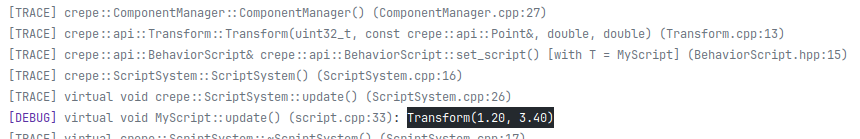
\includegraphics[scale=0.7]{img/poc-output-scripts.png}}
	\caption{Script system \glsfmtshort{poc} output}
	\label{fig:poc-output-scripts}
\end{figure}

\subsection{Logging utilities}
\label{poc:log}

A small \gls{poc} was written to test the engine's logging functions \autocite[log
example]{crepe:code-repo}. The following calls are used in this example:

\begin{blockcode}
dbg_trace();                                 // the dbg_* macros automatically show
dbg_logf("test printf parameters: %d", 3);   // where the message is coming from
logf(LogLevel::INFO,    "info message");
logf(LogLevel::WARNING, "warning");
logf(LogLevel::ERROR,   "error");
\end{blockcode}

The output of this test is shown in \cref{fig:poc-log}.

\begin{figure}
	\centering
	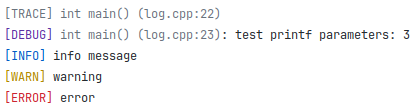
\includegraphics[scale=0.7]{img/poc-log.png}
	\caption{Logging function outputs}
	\label{fig:poc-log}
\end{figure}

\subsection{Audio}
\label{poc:audio}

A test that consists of the following steps was written for each audio library
mentioned in \cref{sec:audio:libs}:\noparbreak
\begin{enumerate}
	\item Load a background track (Ogg Vorbis)
	\item Load three short samples (WAV)
	\item Start the background track
	\item Play each sample sequentially while pausing and resuming the background track
	\item Play all samples simultaniously
	\item Stop all audio and exit
\end{enumerate}

The repository \autocite{crepe:code-repo} contains two finished \glspl{poc} under the
\codeinline{mwe/audio/} subdirectory for miniaudio and SoLoud. The SoLoud \gls{poc}
was later converted to a full audio \gls{facade}, which is currently part of the
cr\^epe engine. The \gls{poc} using the audio \gls{facade} is available from the same
repository, under the \codeinline{src/example/audio_internal.cpp} file.

\subsection{Gameloop}
\label{poc:gameloop}

\begin{figure}
	\centering
	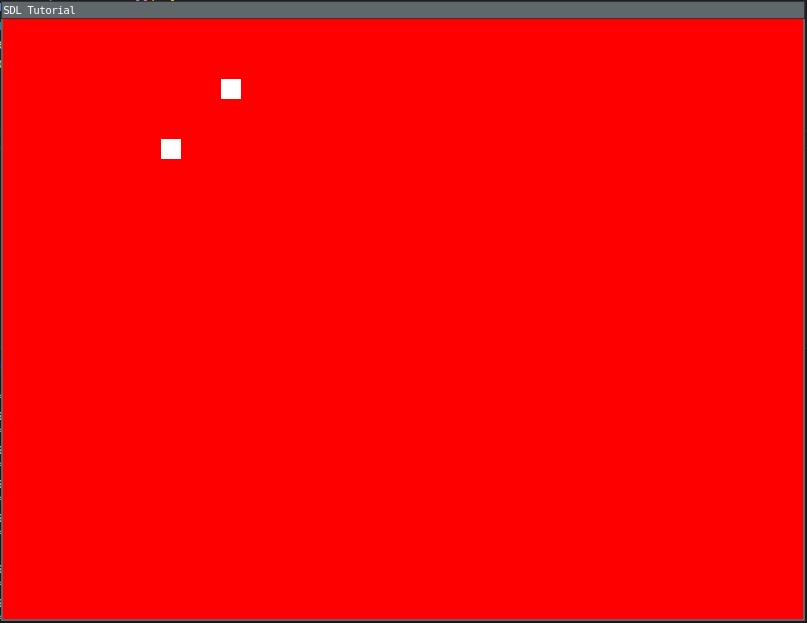
\includegraphics[scale=0.4]{img/gameloop-squares.png}
	\caption{Gameloop running example}
	\label{fig:poc-gameloop-squares}
\end{figure}

This \gls{poc} shows the functionality of the different loops and the approaches to
decouple the updates from the framerate. \Cref{fig:poc-gameloop-squares} shows two
squares that keep moving at the same speed no matter how high or low the framerate
gets. This is done by updating the squares in the per frame update loop with the
delta time generated by the timer. By multipling deltaTime to the velocity of the
square the velocity is converted to a time instead of frames. this can be seen in de
following code example\noparbreak
\begin{blockcode}
float delta = timer.getDeltaTime(); // get delta time of current frame
	if (obj->direction == 1) {
		obj->setX(obj->getX() + 50 * delta); // multiply velocity by delta time for consistent behavior.
	} else {
		obj->setX(obj->getX() - 50 * delta);
	}
\end{blockcode}

The second functionality this \gls{poc} shows is how the fixed loop is executed.
Based on the framerate of the gameloop the fixed loop is executed multiple times per
frame or skips a certain amount of frames as seen in
\cref{fig:poc-gameloop-500fps,fig:poc-gameloop-10fps}.

\begin{figure}
	\centering
	\begin{subfigure}[b]{0.45\textwidth}
		\centering
		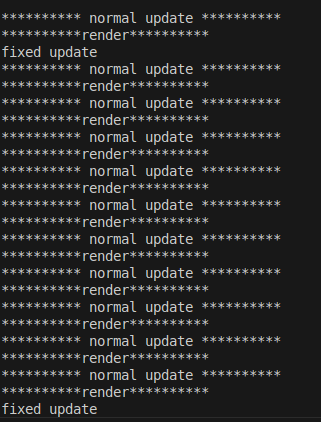
\includegraphics[scale=0.5]{img/gameloop-console.png}
		\caption{Fixed loop (50Hz) with 500 fps}
		\label{fig:poc-gameloop-500fps}
	\end{subfigure}
	\hfill
	\begin{subfigure}[b]{0.45\textwidth}
		\centering
		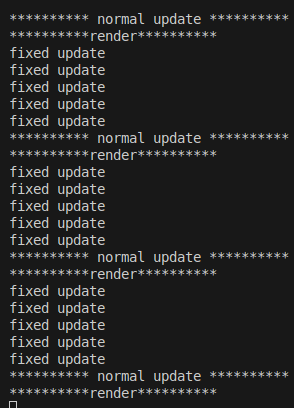
\includegraphics[scale=0.5]{img/gameloop-console-10.png}
		\caption{Fixed loop (50Hz) with 10 fps}
		\label{fig:poc-gameloop-10fps}
	\end{subfigure}
	\caption{Comparison of game loop performance at different frame rates}
	\label{fig:poc-gameloop-console-comparison}
\end{figure}

\subsection{Events/input system}
\label{poc:event}

\begin{figure}
	\centering
	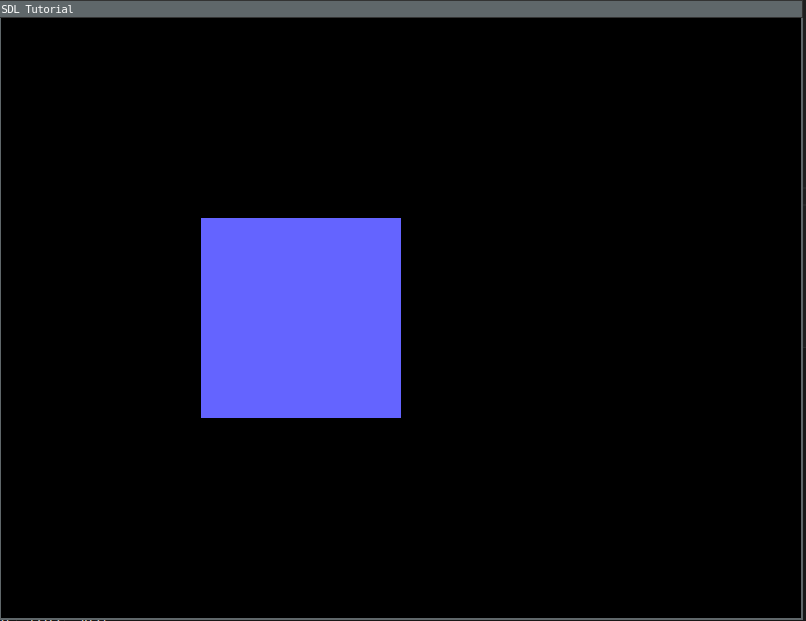
\includegraphics[scale=0.4]{img/poc-button.png}
	\caption{Gameloop running example}
	\label{fig:poc-event}
\end{figure}

The event/input system \gls{poc} shows the different ways the event system can be
used. It also serves as a basis on which the input system is developed. the first two
features show the workings of the two interfaces which are created so the game
developer doesnt need to subscribe each function individualy. The gamedeveloper only
needs to create a derived class from the parent IKeyListener or IMouseListener and
override the functions with their own implementation as shown below.\noparbreak
\begin{description}
	\item[KeyListener] \codeinline{KeyListenerTest keyListener(testListenerId);} this
		line creates a concrete KeyListener that has been created as follows.
		\begin{blockcode}
		class KeyListenerTest : public IKeyListener {
		public:
			KeyListenerTest(int listenerId);
			~KeyListenerTest();

			void onKeyPressed(const KeyPressedEvent& event) override;
			void onKeyReleased(const KeyReleasedEvent& event) override;
		};
		\end{blockcode}
		The functions have been overridden to add custom functionality, which is called
		when a key is pressed or released.
	\item[MouseListener] Like the KeyListener, \codeinline{MouseListenerTest
		mouseListener(testListenerId);} is a concrete derived class of IMouseListener,
		created as follows:\noparbreak
		\begin{blockcode}
		class MouseListenerTest : public IMouseListener {
		public:
			MouseListenerTest(int listenerId);
			~MouseListenerTest();

			void onMouseClicked(const MouseClickEvent& event) override;
			void onMousePressed(const MousePressedEvent& event) override;
			void onMouseReleased(const MouseReleasedEvent& event) override;
			void onMouseMoved(const MouseMovedEvent& event) override;
		};
		\end{blockcode}
\end{description}

Secondly the \gls{poc} shows how the gamedeveloper can create custom events by
creating a derived class from the parent class Event. This custom event can then be
used to subscribe callbacks to which can use the data within the derived class. Below
is an example of such a custom event.\noparbreak
\begin{blockcode}
class PlayerDamagedEvent : public Event {
public:
	PlayerDamagedEvent(int damage, int playerID)
		: Event("PlayerDamaged"), damage(damage), playerID(playerID) {}

	REGISTER_EVENT_TYPE(PlayerDamagedEvent);

    int getDamage() const { return damage; }
    int getPlayerID() const { return playerID; }

private:
	int damage;
	int playerID;
};
\end{blockcode}

An example of a callback function using the custom PlayerDamagedEvent:\noparbreak
\begin{blockcode}
void onPlayerDamaged(const PlayerDamagedEvent & e) {
	std::cout << "Player " << e.getPlayerID() << " took " << e.getDamage()
				<< " damage." << std::endl;
}
\end{blockcode}

Lastly the \gls{poc} shows how a button can be handled using a input sytem. The blue
square in \cref{poc:event} represents a button component which will call its
onClick() function when the mouse click event triggers within its boundary. The
result can be seen in \cref{fig:poc-event-button}.

\begin{figure}
	\centering
	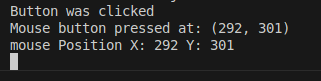
\includegraphics[scale=1]{img/poc-event-button.png}
	\caption{gameloop running example}
	\label{fig:poc-event-button}
\end{figure}

\subsection{Camera}
\label{poc:camera}

The camera \gls{poc} \autocite[camera example]{crepe:code-repo} consists of the
following:\noparbreak
\begin{itemize}
	\item An \codeinline{on_key_pressed} function, which listens for key presses and
		adjusts camera position and zoom based on key inputs.
	\item A user-defined script class (\codeinline{MyCameraScript}) derived from
		\codeinline{Script}, implementing only the \codeinline{update()} function. To
		update the camera movements and zoom.
	\item A main function that---
		\begin{itemize}
			\item Subscribes the \codeinline{on_key_pressed} function to handle
				\codeinline{KeyPressedEvent} events.
			\item Creates a \codeinline{GameObject} for the camera and adds
				\codeinline{Camera} and \codeinline{BehaviorScript} components, with
				\codeinline{MyCameraScript} attached to manage the camera's transformation.
			\item Instantiates a background \codeinline{GameObject} with
				\codeinline{Transform} and \codeinline{Sprite} components, loading an
				external texture as its background.
		\end{itemize}
\end{itemize}

Running this \gls{poc} allows for controlled camera movement and zoom in response to
key inputs. The \codeinline{MyCameraScript::update} function ensures that these
transformations are applied each frame, as demonstrated by the output in
\cref{fig:poc-output-camera}.

\begin{figure}
	\centering
	\fitimg{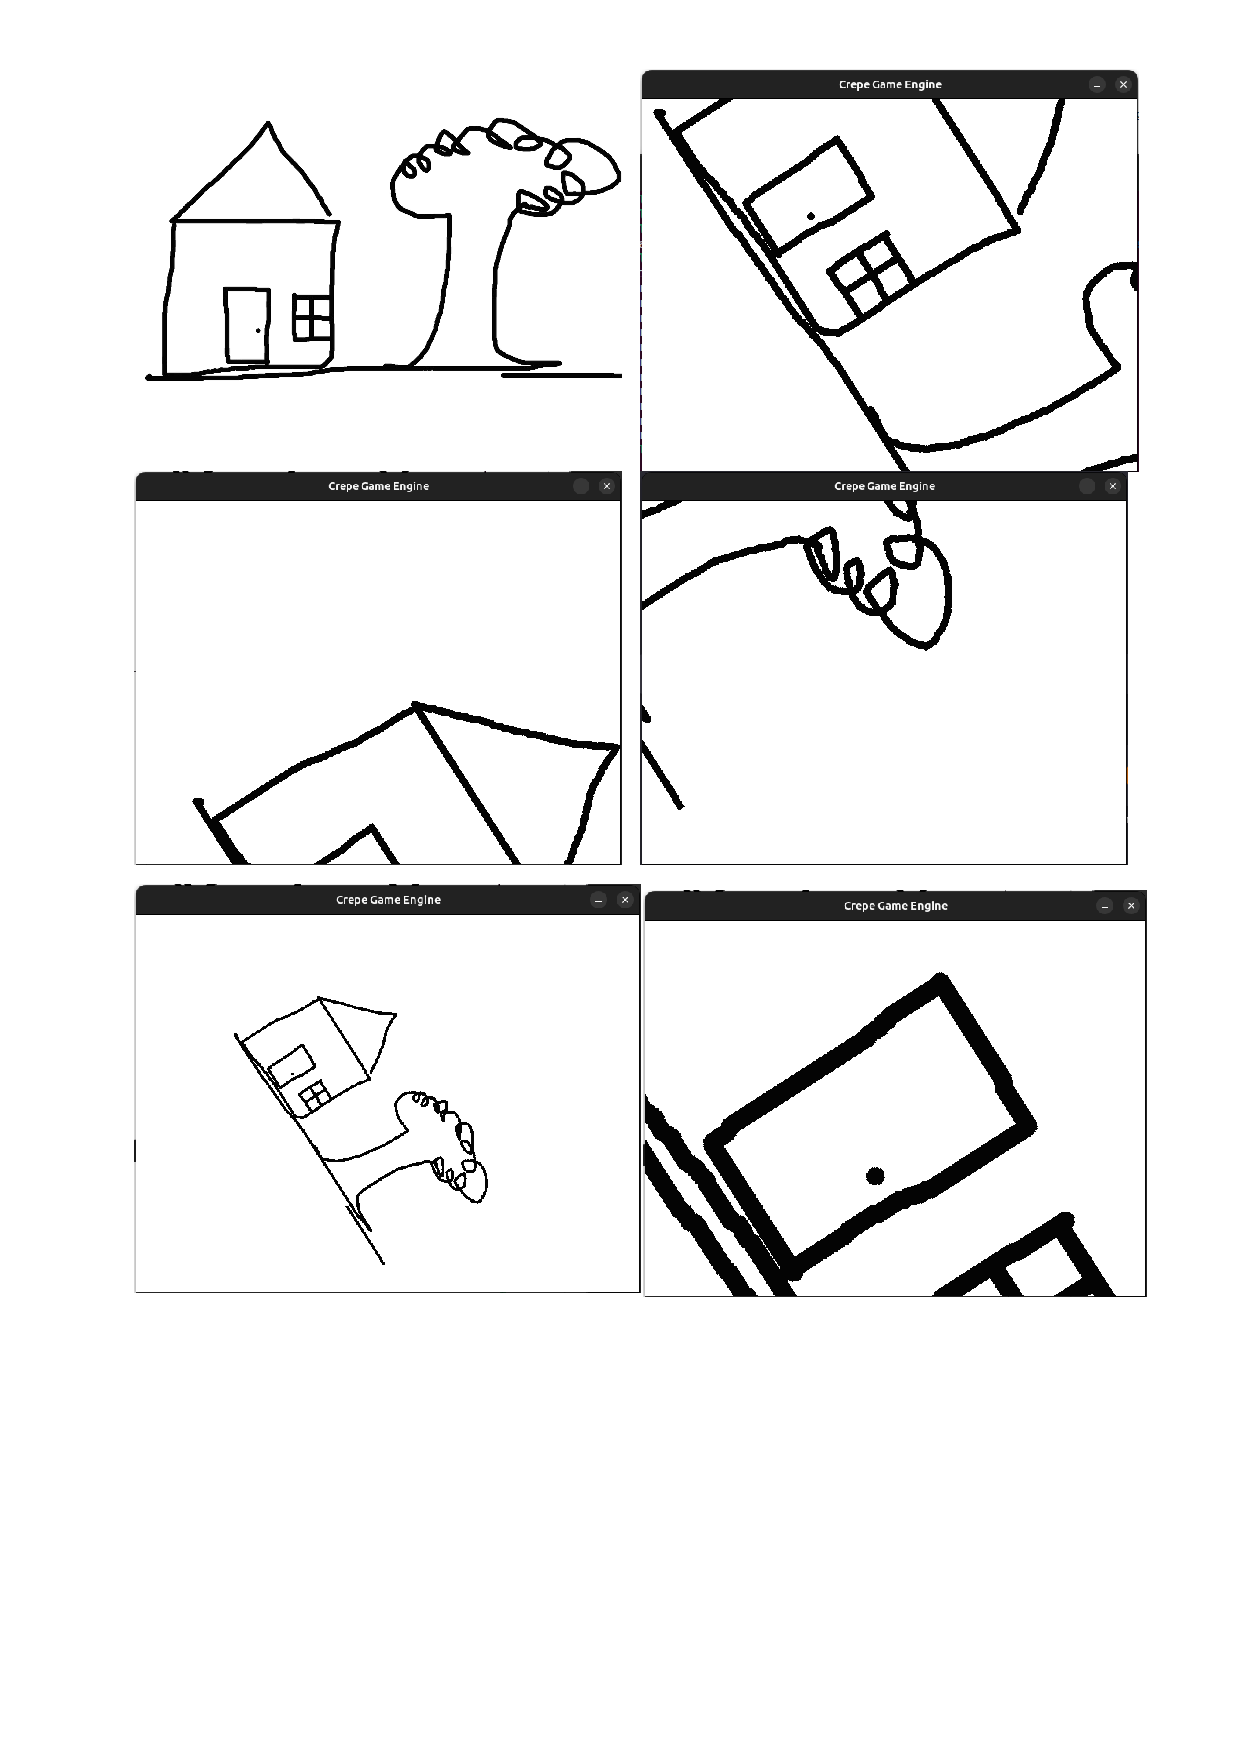
\includegraphics[scale=0.7]{img/poc-camera.pdf}}
	\caption{Camera \glsfmtshort{poc} output}
	\label{fig:poc-output-camera}
\end{figure}

\makeatletter%
\newbox\full@class@diag%
\newlength\full@class@diag@width%
\newlength\full@class@diag@height%
\savebox\full@class@diag{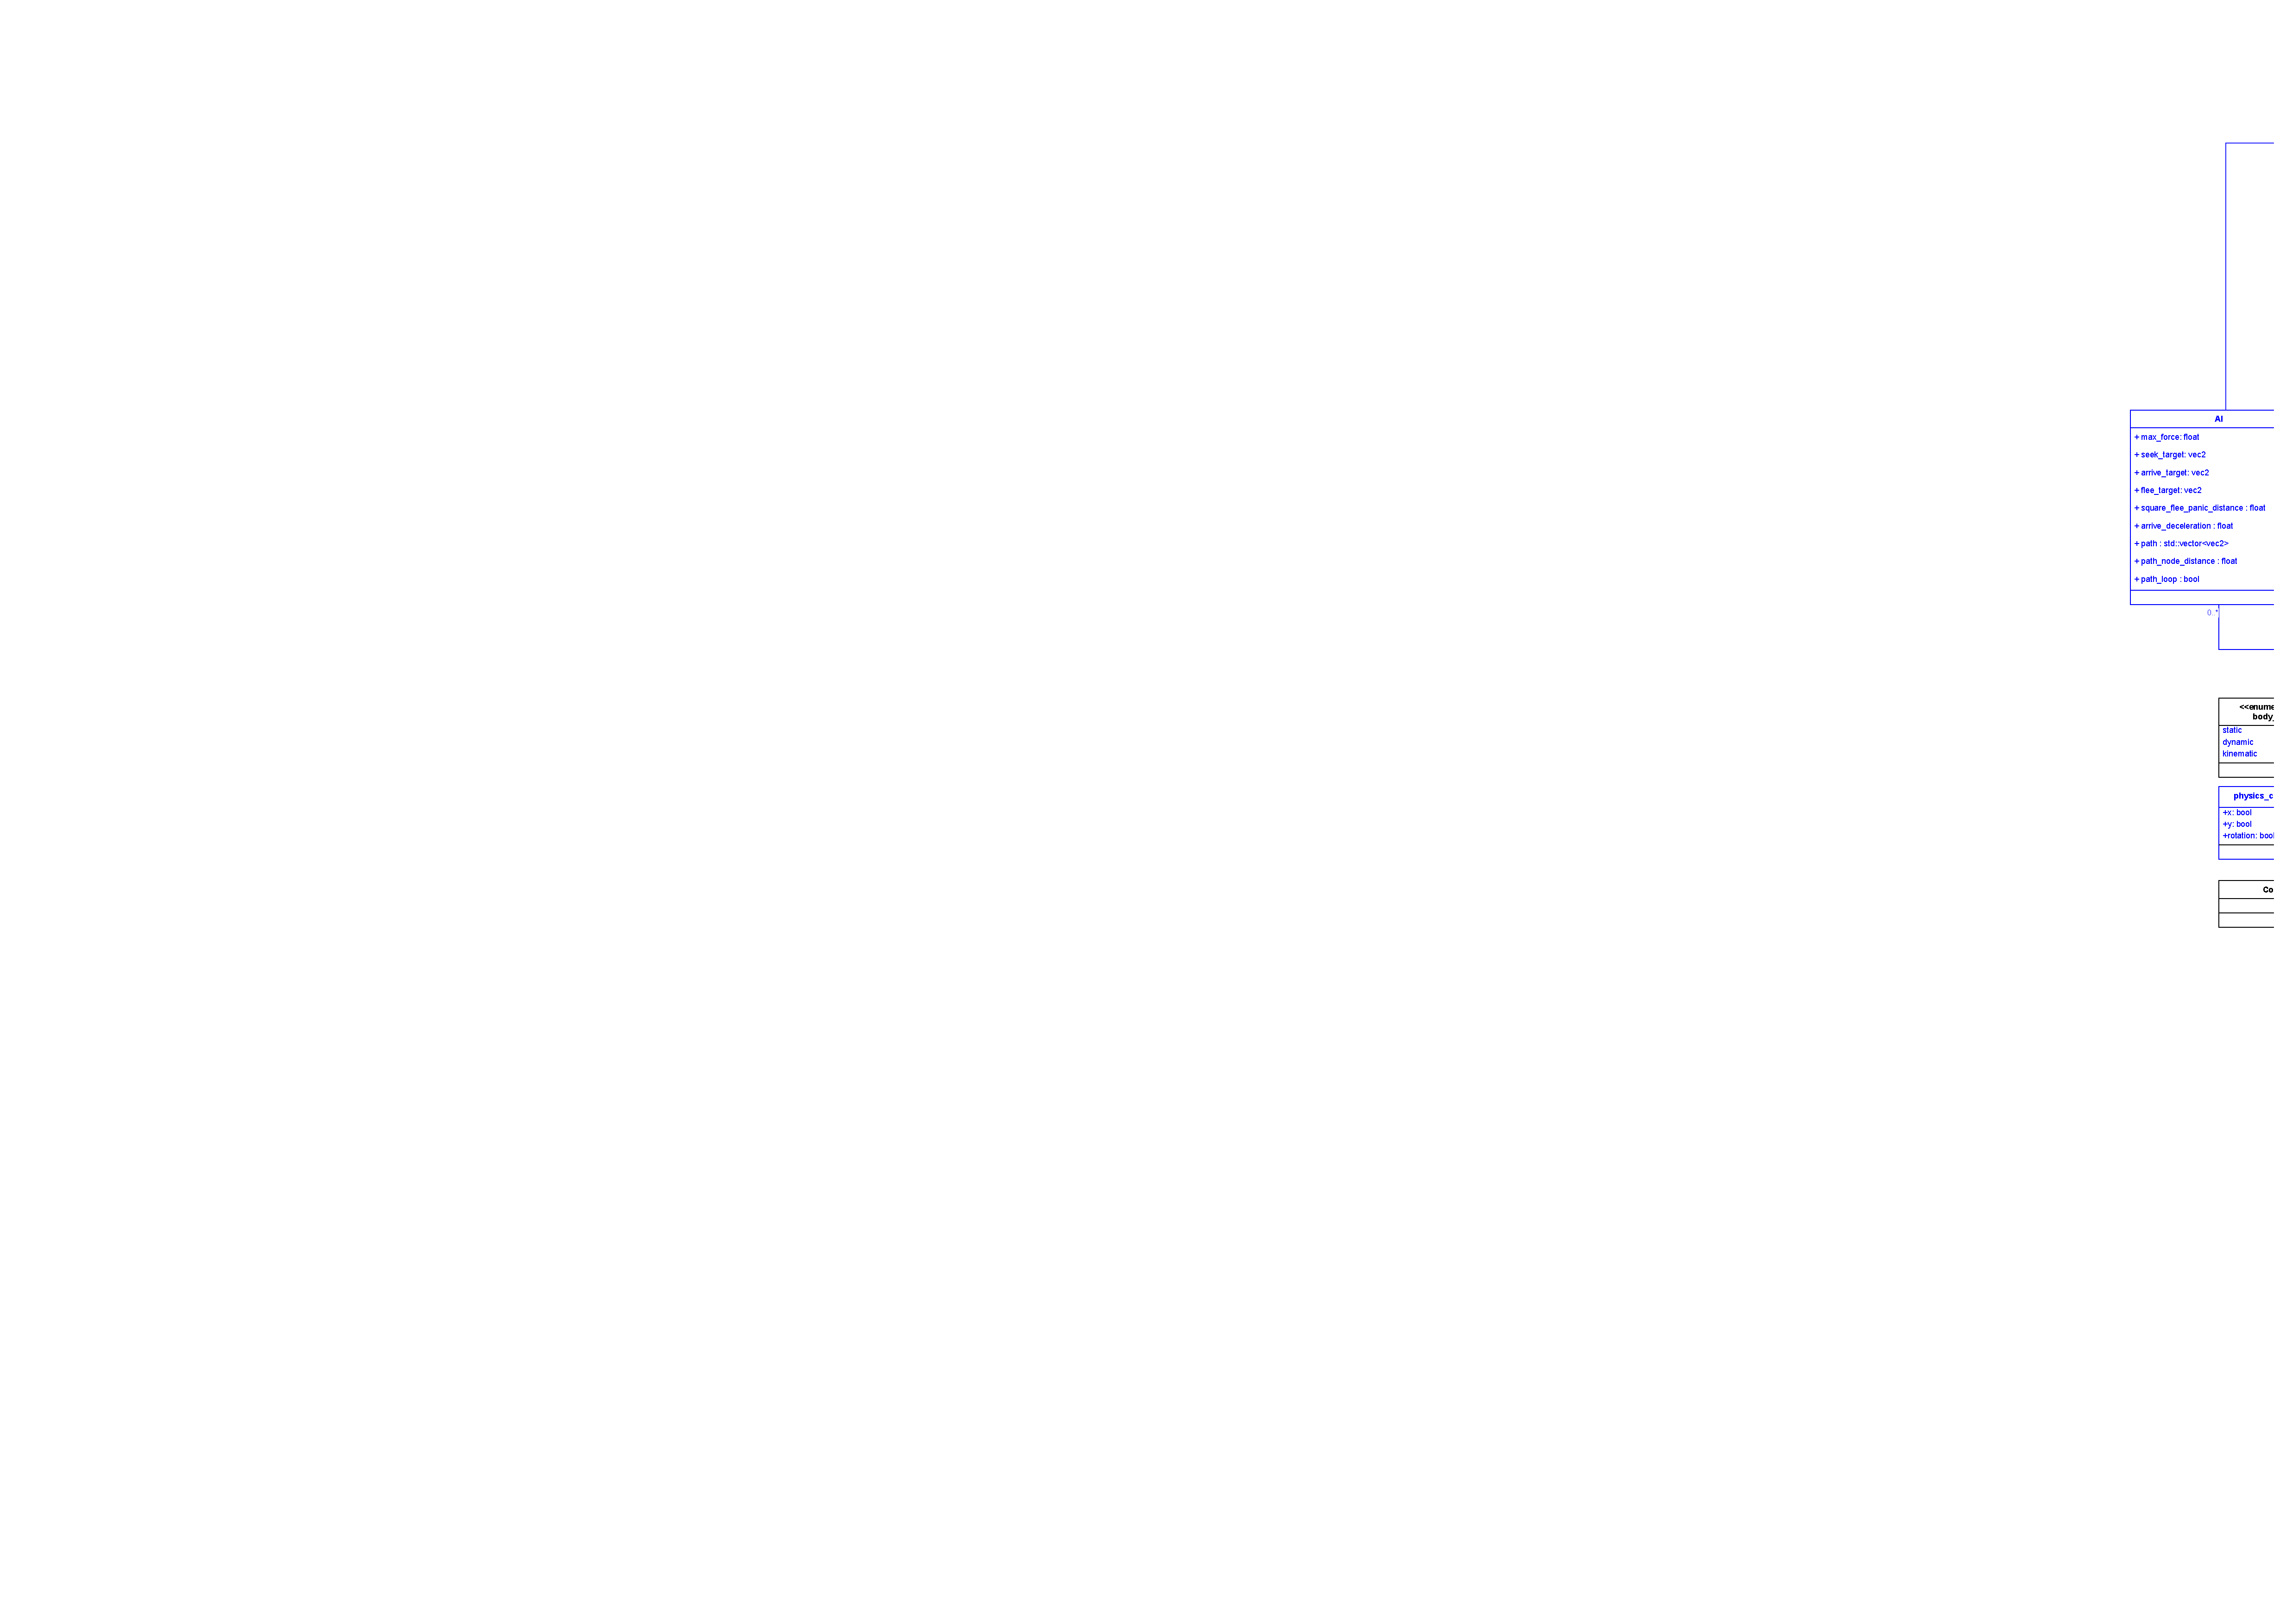
\includegraphics{img/class-api-full.pdf}}%
\settowidth\full@class@diag@width{\usebox\full@class@diag}%
\settoheight\full@class@diag@height{\usebox\full@class@diag}%
\begingroup%
\eject%
\thispagestyle{empty}%
\pdfpagewidth=\full@class@diag@width%
\pdfpageheight=\full@class@diag@height%
\AddToShipoutPictureBG*{%
  \AtPageUpperLeft{%
		\raisebox{-\full@class@diag@height}{%
			\usebox\full@class@diag%
		}%
	}%
}%
\section{Full API class diagram}%
\newpage%
\endgroup%
\makeatother%

\end{document}

